\documentclass[oneside]{article}

\usepackage[utf8]{inputenc}
\usepackage[english]{babel}
\usepackage{graphicx}
\usepackage{geometry}
\usepackage{listings}
\usepackage{color}
\usepackage{fancyhdr}

\geometry {
a4paper,
total={170mm,257mm},
top=25mm,
right=20mm,
bottom=20mm,
left=20mm
}

\definecolor{dkgreen}{rgb}{0,0.6,0}
\definecolor{gray}{rgb}{0.5,0.5,0.5}
\definecolor{mauve}{rgb}{0.58,0,0.82}

\lstset{frame=tb,
  language=C++,
  aboveskip=3mm,
  belowskip=3mm,
  showstringspaces=false,
  columns=flexible,
  basicstyle={\small\ttfamily},
  numbers=left,
  numberstyle=\tiny\color{gray},
  keywordstyle=\color{blue},
  commentstyle=\color{dkgreen},
  stringstyle=\color{mauve},
  breaklines=true,
  breakatwhitespace=true,
  tabsize=4,
  frame=single
}

\pagestyle{fancy}
\fancyhf{}
\rhead{\thepage}
\lhead{ACM ICPC Reference}
\cfoot{.++}

\begin{document}

\begin{titlepage}
  \centering
  
\includegraphics[width=0.15\textwidth]{logo.png}\par\vspace{1cm}
  {\scshape\LARGE Universidade Federal de Itajubá \par}
  \vspace{1.5cm}
  {\huge\bfseries ACM ICPC Reference\par}
  \vspace{2cm}
  {\scshape\Large .++\par}  
  \vspace{1cm}
  {\Large\itshape Dêner José Ribeiro\par}
  {\Large\itshape Eduardo Augusto de Oliveira\par}
  {\Large\itshape Leonardo Furtado de Oliveira\par}
  \vfill
  Coaches\par
  ~Felipe Kallás Silva
  
  \vfill
  
  {\large Junho / 2019\par}
\end{titlepage}

\thispagestyle{empty}
\tableofcontents
\pagebreak

\textbf{* The codes listed below use the following header.}
\begin{lstlisting}
#include <bits/stdc++.h>

using namespace std;

#define ii pair<int, int>
#define vi vector<int>
#define vii vector<ii>
#define vb vector<bool>
#define ll long long
#define mk make_pair
#define pb push_back
#define MAXN *
\end{lstlisting}
* Problem limit

\section{Graphs and Trees}

\subsection{Depth-First Search (DFS)}
Time: $O(V + E)$
\begin{lstlisting}
int n;
vi graph[MAXN];
bool vis[MAXN];

void dfs(int u) {
    vis[u] = true;
    for (int v : graph[x])
    	if (!vis[v])
    		dfs(v);
}
\end{lstlisting}

\subsection{Breadth-First Search (BFS)}
Time: $O(V + E)$
\begin{lstlisting}
int n;
vi graph[MAXN];

vi bfs(int src, int w = 1) {
    queue<int> q;
    vi dist(n, INT_MAX);
    vb vis(n);

    q.push(src);
    dist[src] = 0;
    while (!q.empty()) {
        int u = q.front();
        q.pop();
        vis[u] = true;
        for (int v : graph[u]) {
            if (!vis[v] && dist[u] + w < dist[v]) {
                dist[v] = dist[u] + w;
                q.push(v);
            }
        }
    }
    return dist;
}
\end{lstlisting}

\subsection{Dijkstra}
Time: $O(n^2logn)$
\begin{lstlisting}
int n;
vii graph[MAXN];

vi dijkstra(int src) {
    priority_queue<ii, vii, greater<ii>> pq;
    vi dist(n, INT_MAX);
    vb vis(n, false);

    pq.push(mk(0, src));
    dist[src] = 0;
    while (!pq.empty()) {
        int u = pq.top().second;
        pq.pop();
        vis[u] = true;
        for (int i : graph[u] {
            int w = i.first;
            int v = i.second;
            if (!vis[v] && dist[v] > dist[u] + w) {
                dist[v] = dist[u] + w;
                pq.push(mk(dist[v], v));
            }
        }
    }
    return dist;
}
\end{lstlisting}

\subsection{Bellman-Ford}
Time: $O(V * E)$
\begin{lstlisting}
struct edge {
    int u, v, w;
    edge() {};
    edge(int _u, int _v, int _w) {
        u = _u, v = _v, w = _w;
    }
};

int n, m;
vector<edge> graph;

bool bellman(int src) {
    vi dist(n, INT_MAX);

    dist[src] = 0;
    for (int i = 0; i < n - 1; i++)
        for (edge e : graph)
            if (dist[e.u] != INT_MAX)
                dist[e.v] = min(dist[e.u] + e.w, dist[e.v]);
    for (edge e : graph)
        if (dist[e.u] != INT_MAX && dist[e.u] + e.w < dist[e.v])
            return true;
    return false;
}
\end{lstlisting}
\pagebreak
\subsection{Kruskal}
Time: $O(nlogn)$
\begin{lstlisting}
struct edge {
    int u, v, w;
    edge() {};
    edge(int _u, int _v, int _w) {
        u = _u, v = _v, w = _w;
    }
    bool operator < (const edge su) const {
        return w < su.w;
    }
};

int n, m, root[MAXN];
vector<edge> graph;

int findset(int u) {
    return root[u] == u ? u : root[u] = findset(root[u]);
}

void initset() {
    for (int i = 0; i < n; i++) root[i] = i;
}

int kruskal() {
    initset();
    sort(graph.begin(), graph.end());
    vi tree[n];
    int total = 0;
    for (int i = 0; i < m; i++) {
        int u = graph[i].u;
        int v = graph[i].v;
        int w = graph[i].w;

        int fu = findset(u);
        int fv = findset(v);
        if (fu != fv) {
            root[fu] = fv;
            total += w;
            tree[u].pb(v);
        }
    }
    return total;
}
\end{lstlisting}

\subsection{Floyd-Warshall}
Time: $O(n^3)$
\begin{lstlisting}
int n, graph[MAXN][MAXN];

void floyd() {
    for (int k = 0; k < n; k++)
        for (int i = 0; i < n; i++)
            for (int j = 0; j < n; j++)
                graph[i][j] = min(graph[i][j], graph[i][k] + graph[k][j]);
}
\end{lstlisting}
* Don't use $INT_-$$MAX$

\subsection{Ford-Fulkerson}
Time: $O(EV^3)$
\begin{lstlisting}
int graph[MAXN][MAXN], parent[MAXN], n;

bool bfs(int src, int snk) {
    vb vis(n);
    queue<int> q;
    q.push(src);

    parent[src] = -1;
    vis[src] = true;
    while (!q.empty()) {
        int u = q.front();
        q.pop();
        vis[u] = true;
        for (int v = 0; v < n; v++)
            if (!vis[v] && graph[u][v]) {
                q.push(v);
                parent[v] = u;
                vis[v] = true;
            }
    }
    return vis[snk];
}

int ford(int src, int snk) {
    int flow = 0;
        
    while (bfs(src, snk)) {
        int path_flow = INT_MAX;
        for (int v = snk; v != src; v = parent[v])
            path_flow = min(path_flow, graph[parent[v]][v]);

        for (int v = snk; v != src; v = parent[v]) {
            graph[parent[v]][v] -= path_flow;
            graph[v][parent[v]] += path_flow;
        }
        flow += path_flow;
    }
    return flow;
}
\end{lstlisting}
\pagebreak
\subsection{Tarjan}
Time: $O(V + E)$
\begin{lstlisting}
int n, disc[MAXN], low[MAXN], scc[MAXN], ct, id;
vi graph[MAXN];
stack<int> st;
bool onstack[MAXN];

void dfs(int u) {
    disc[u] = low[u] = ct++;
    st.push(u);
    onstack[u] = true;

    for (int v : graph[u]) {
        if (disc[v] == -1) {
            dfs(v);
            low[u] = min(low[u], low[v]);
        } else if (onstack[v])
            low[u] = min(low[u], disc[v]);
    }
    if (low[u] == disc[u]) {
        int v;
        do {
            v = st.top();
            st.pop();
            onstack[v] = false;
            scc[v] = id;
        } while (u != v);
        id++;
    }
}

void tarjan() {
    ct = id = 0;
    memset(disc, -1, sizeof disc);
    for (int i = 0; i < n; i++)
        if (disc[i] == -1)
            dfs(i);
}
\end{lstlisting}

\subsection{Fenwick Tree}
Time: $O(logn)$
\begin{lstlisting}
int n, bit[MAXN], v[MAXN];

int query(int i) {
    int sum = 0;
    for (; i > 0; i -= i & (-i))
        sum += bit[i];
    return sum;
}

void update(int i, int value) {
    for (; i <= n; i += i & (-i))
        bit[i] += value;
}

void build() {
    memset(bit, 0, sizeof bit);
    for (int i = 1; i <= n; i++)
        update(i, v[i-1]);
}
\end{lstlisting}
\pagebreak
\subsection{Segment Tree}
Build Time: $O(n)$ $|$ Query Time: $O(logn)$ $|$ Update Time: $O(logn)$
\begin{lstlisting}
int v[MAXN], st[4 * MAXN], /* lazy[4 * MAXN] */;

void build(int l, int r, int no = 0) {
    if (l > r) return;
    if (l == r) {
        st[no] = v[l];
        return;
    }
    int mid = l + (r - l) / 2;
    build(l, mid, no * 2 + 1);
    build(mid + 1, r, no * 2 + 2);
    st[no] = st[no * 2 + 1] + st[no * 2 + 2];
}

/* void prop(int l, int r, int no) {
    if (lazy[no] != 0) {
        st[no] += (r - l + 1) * lazy[no];
        if (l != r) {
            lazy[no * 2 + 1] += lazy[no];
            lazy[no * 2 + 2] += lazy[no];
        }
        lazy[no] = 0;
    }
} */

int query(int l, int r, int qs, int qe, int no = 0) {    
    if (l > r || l > qe || r < qs) return 0;
    // prop(l, r, no);
    if (l >= qs && r <= qe) return st[no];
    int mid = l + (r - l) / 2;
    return query(l, mid, qs, qe, 2 * no + 1) + query(mid + 1, r, qs, qe, 2 * no + 2);
}

void update(int l, int r, int value, int pos, int no = 0) {
    if (l > pos || r < pos) return;
    st[no] += value;
    if (l == r) return;
    int mid = l + (r - l) / 2;
    update(l, mid, value, pos, no * 2 + 1);
    update(mid + 1, r, value, pos, no * 2 + 2);
}

/* void lazyUpdate(int l, int r, int qs, int qe, int value, int no = 0) {
    if (l > r || l > qe || r < qs) return;
    prop(l, r, no);
    if (l >= qs && r <= qe) {
        st[no] += (r - l + 1) * value;
        if (l != r) {
            lazy[no * 2 + 1] += value;
            lazy[no * 2 + 2] += value;
        }
        return;
    }
    int mid = l + (r - l) / 2;
    lazyUpdate(l, mid, qs, qe, value, no * 2 + 1);
    lazyUpdate(mid + 1, r, qs, qe, value, no * 2 + 2);
    st[no] = st[no * 2 + 1] + st[no * 2 + 2];
} */
\end{lstlisting}
* Lazy propagation commented.
\pagebreak
\section{Dynamic Programming}

\subsection{Merge-Sort}
Time: $O(nlogn)$
\begin{lstlisting}
int merge(int v[], int l, int r) {
    if (r == l)
        return 0;
    int invs = 0, mid = l + (r - l) / 2;

    invs += merge(v, l, mid);
    invs += merge(v, ++mid, r);

    int i = l, j = mid;
    queue<int> temp;

    while (i <= mid - 1 && j <= r) {
        if (v[i] <= v[j])
            temp.push(v[i++]);
        else {
            temp.push(v[j++]);
            invs += (mid - i);
        }
    }
    while (i <= mid - 1)
        temp.push(v[i++]);
    while (j <= r)
        temp.push(v[j++]);
    for (i = l; i <= r; i++) {
        v[i] = temp.front();
        temp.pop();
    }
    return invs;
}
\end{lstlisting}

\subsection{Longest Increasing Subsequence (LIS)}
Time: $O(n)$
\begin{lstlisting}
int n, v[MAXN];

int lis() {
    if (!n)
        return 0;
    vi tail(n), prev(n, -1);
    int len = 1;

    for (int i = 1; i < n; i++) {
        if (v[i] < v[tail[0]])
            tail[0] = i;
        else if (v[i] > v[tail[len - 1]]){
            prev[i] = tail[len - 1];
            tail[len++] = i;
        } else {
            int pos = distance(tail.begin(), upper_bound(tail.begin(), tail.begin() + len - 1, v[i]));
            prev[i] = tail[pos - 1];
            tail[pos] = i;
        }
    }
    return len;
}
\end{lstlisting}

\subsection{Longest Common Subsequence (LCS)}
Time: $O(n * m)$
\begin{lstlisting}
string s, t;

int lcs() {
    int n = s.size(), m = t.size();
    int dp[n + 1][m + 1];
    
    for (int i = 0; i <= n; i++) {
        for (int j = 0; j <= m; j++) {
            if (!i || !j)
                dp[i][j] = 0;
            else if (s[i - 1] == t[j - 1])
                dp[i][j] = dp[i - 1][j - 1] + 1;
            else
                dp[i][j] = max(dp[i - 1][j], dp[i][j - 1]);
        }
    }
    return dp[n][m];
    
    /* int i = n, j = m, index = dp[n][m];
    string seq(n + 1, ' ');
    while (i > 0 && j > 0) {
        if (s[i - 1] == t[j - 1]) {
            i--; j--; index--;
            seq[index] = s[i];
        } else if (dp[i - 1][j] > dp[i][j - 1])
            i--;
        else
            j--;
    }
    return seq; */
}
\end{lstlisting}
* Sequence building commented.

\subsection{Kadane}
Time: $O(n)$
\begin{lstlisting}
int v[MAXN];
// Max interval sum
int kadane() {
    int max = INT_MIN, temp = 0;
    for (int i : v) {
        temp += i;
        if (max < temp) max = temp;
        if (temp < 0) temp = 0;
    }
    return max;
}
\end{lstlisting}
\pagebreak
\subsection{Knapsack}
Time: $O(n * w)$
\begin{lstlisting}
int value[MAXN], weight[MAXN];
// Minimum sum of elements in which the sum of weights is less than or equal to w
int knapsack(int n, int w) {
   int dp[n + 1][w + 1];
   for (int i = 0; i <= n; i++) {
        for (int j = 0; j <= w; j++) {
            if (!i || !j)
                dp[i][j] = 0;
            else if (weight[i - 1] <= j)
                dp[i][j] = max(value[i - 1] + dp[i - 1][j - weight[i - 1]],  dp[i - 1][j]);
            else
                dp[i][j] = dp[i - 1][j];
        }
    }
    return dp[n][w];
}
// With repetitions
int unbKnapsack(int n, int w) {
    vi dp(w + 1);
    for (int i = 1; i <= w; i++)
        for (int j = 0; j < n; j++)
            if (weight[j] <= i)
                dp[i] = max(dp[i - weight[j]] + value[j], dp[i]);
    return dp[w];
}
\end{lstlisting}

\subsection{Coin Change}
Time: $O(n * w)$
\begin{lstlisting}
int coins[MAXN];

int minCoins(int n, int w) {
    vi dp(w + 1, INT_MAX);
    dp[0] = 0;

    for (int i = 1; i <= w; i++) {
        for (int j = 0; j < n; j++) {
            if (coins[j] <= i) {
                int sub_res = dp[i - coins[j]];
                if (sub_res != INT_MAX && sub_res + 1 < dp[i])
                    dp[i] = sub_res + 1;
            }
        }
    }
    return dp[w];
}
// Total possibilities
int count(int n, int w) {
    if (!w)
        return 1;
    if (w < 0)
        return 0;        
    if (n <= 0 && w >= 1)
        return 0;
    return count(n - 1, w) + count(n, w - coins[n - 1]);
}
\end{lstlisting}

\pagebreak
\section{Math and Geometry}

\subsection{Greatest Common Divisor}
Time: $O(log(min(x, y)))$
\begin{lstlisting}
int gcd(int x, int y) {
	return y ? gcd(y, x % y) : abs(x);
}
\end{lstlisting}

\subsection{Least Common Multiple}
Time: $O(gcd(x, y))$
\begin{lstlisting}
int lcm(int x, int y) {
	if (x && y) return abs(x) / gcd(x, y) * abs(y);
	return abs(x | y);
}
\end{lstlisting}

\subsection{Extended Euclidean Algorithm}
Time: $O(log(min(x, y)))$
\begin{lstlisting}
int egcd(int a, int b, int &x, int &y) {
    if (a == 0) {
        x = 0, y = 1;
        return b;
    }
    int xo, yo;
    int gcd = egcd(b % a, a, xo, yo);
    x = yo - (b / a) * xo;
    y = xo;
    if (gcd < 0)
        gcd = -gcd, x = -x, y = -y;
    return gcd;
}
\end{lstlisting}

\subsection{N Choose R}
Time: $O(p^2 * log_p{n})$
\begin{lstlisting}
int ncrDp(int n, int r, int p) {
    vi dp(r + 1);
    dp[0] = 1;
    for (int i = 1; i <= n; i++)
        for (int j = min(i, r); j > 0; j--)
            dp[j] = (dp[j] + dp[j - 1]) % p;
    return dp[r];
}

int ncr(int n, int r, int p) {
    if (!r)
        return 1;
    return (ncr(n / p, r / p, p) * ncrDp(n % p, r % p, p)) % p;
}
\end{lstlisting}
\pagebreak
\subsection{Modular Multiplication}
Time: $O(logn)$
\begin{lstlisting}
int mulmod(int a, int b, int p = 1e9+7) {
    int x = 0;
    a %= p;
    while (b > 0) {
        if (b & 1)
            x = (x + a) % p;
        a = (a * 2) % p;
        b >>= 1;
    }
    return x % p;
}
\end{lstlisting}

\subsection{Modular Exponentiation}
Time: $O(logn)$
\begin{lstlisting}
int expmod(int a, int b, int p = 1e9+7) {
    int x = 1;
    a %= p;
    while (b > 0) {
        if (b & 1)
            x = (x * a) % p;        
        a = (a * a) % p;
        b >>= 1;
    }
    return x;
}
\end{lstlisting}

\subsection{Modular Inverse}
Time: $O(log(min(x, y)))$
\begin{lstlisting}
int invmod(int a, int p = 1e9+7) {
    int x, y;
    int gcd = egcd(a, p, x, y);
    if (gcd != 1) return -1;
    return x % p + ((x < 0) ? p : 0);
}
\end{lstlisting}

\subsection{Matrix Multiplication}
Time: $O(n^3)$
\begin{lstlisting}
struct matrix {
    int mat[MAXN][MAXN];
};

int n;

matrix matMul(matrix a, matrix b) {
    matrix c;
    int k;
    for (int i = 0; i < n; i++)
        for (int j = 0; j < n; j++)
            for (c.mat[i][j] = k = 0; k < n; k++)
                c.mat[i][j] += a.mat[i][k] * b.mat[k][j];
    return c;
}
\end{lstlisting}

\subsection{Sieve Of Eratosthenes}
Time: $O(n)$
\begin{lstlisting}
// Primes from 2 to n
vi sieve(int n) {
    vb prime(n + 1, true);
    
    for (int p = 2; p * p <= n; p++)
        if (prime[p])
            for (int i = p * 2; i <= n; i += p)
                prime[i] = false;
	vi v;
    for (int p = 2; p <= n; p++)
        if (prime[p])
    		v.pb(p);
	return v;
}
\end{lstlisting}

\subsection{Factoring}
Time: $O(\sqrt{n})$
\begin{lstlisting}
vi factorize(int n) {
	vi v;
	for(int i = 2; i * i <= n; i++) {
		if (n % i) continue;
		v.pb(i);
		n /= i--;
	}
	if (n > 1) v.pb(n);
	return v;
}
\end{lstlisting}

\subsection{Divisors}
Time: $O(\sqrt{n})$
\begin{lstlisting}
vi divisors(int n) {
	int maxP = sqrt(n) + 2;
	vi div;
	for (int i = 1; i <= maxP; i++) {
		if (n % i == 0) {
			div.pb(i);
			div.pb(n / i);
		}
	}
	return div;
}
\end{lstlisting}

\subsection{Amount of Divisors}
Time: $O(n^2)$
\begin{lstlisting}
// Amount of divisors of each integer from 0 to n
vi amount(int n) {
	vi v(n + 1);
	for (int i = 1; i <= n; i++)
		for (int j = i; j <= n; j += i)
			v[j]++;
	return v;
}
\end{lstlisting}

\subsection{Polygon Area}
Time: $O(n)$
\begin{lstlisting}
int n;
double x[MAXN], y[MAXN];
// Points need to be given a clockwise or anti-clockwise manner.
double area() {
    double total = 0;
    int j = n - 1;
    for (int i = 0; i < n; i++) {
        total += (x[j] + x[i]) * (y[j] + y[i]);
        j = i;
    }
    return (total >= 0) ? (total / 2) : (-total / 2);
}
\end{lstlisting}

\subsection{Convex Hull}
Time: $O(nlogn)$
\begin{lstlisting}
struct Point {
    int x, y;
    Point () {}
    Point (int _x, int _y) {
        x = _x, y = _y;
    }
};

int n;
Point points[MAXN], p0;

Point nextToTop(stack<Point> &S) {
    Point p = S.top();
    S.pop();
    Point res = S.top();
    S.push(p);
    return res;
}

int distSq(Point p1, Point p2) {
    return pow(p1.x - p2.x, 2) + pow(p1.y - p2.y, 2);
}
  
int orientation(Point p, Point q, Point r) {
    int val = (q.y - p.y) * (r.x - q.x) - (q.x - p.x) * (r.y - q.y);
    if (val == 0) return 0;
    return (val > 0)? 1 : 2;
}

int compare(Point a, Point b) {
    int o = orientation(p0, a, b);
    if (!o)
        return (distSq(p0, b) >= distSq(p0, a));
    return (o == 2);
}

double convexHull() {
    int ymin = points[0].y, min = 0;
    for (int i = 1; i < n; i++) {
        int y = points[i].y;
        if ((y < ymin) || (ymin == y && points[i].x < points[min].x))
            ymin = points[i].y, min = i;
    }

    swap(points[0], points[min]);

    p0 = points[0];
    sort(points + 1, points + n, compare);

    int m = 1;
    for (int i = 1; i < n; i++) {
        while (i < n-1 && !orientation(p0, points[i], points[i+1]))
            i++;
        points[m++] = points[i];
    }

    if (m < 3) return 0;

    stack<Point> S;
    S.push(points[0]);
    S.push(points[1]);
    S.push(points[2]);

    for (int i = 3; i < m; i++) {
        while (orientation(nextToTop(S), S.top(), points[i]) != 2)
            S.pop();
        S.push(points[i]);
    }

    double total = 0;
    Point ant = S.top(), prim = S.top();
    S.pop();
    while (!S.empty()) {
        total += sqrt(distSq(S.top(), ant));
        ant = S.top();
        S.pop();
    }
    total += sqrt(distSq(ant, prim));
    return total;
}
\end{lstlisting}
\pagebreak

\section{Templates}

\subsection{Point}
\begin{lstlisting}
struct Point {
	double x, y;
	Point () {}
	Point (double _x, double _y) {
		x = _x; y = _y;
    }
    
	Point operator +(const Point & other) const {
		return Point (x + other.x, y + other.y);
	}
	Point operator -(const Point & other) const {
		return Point (x - other.x, y - other.y);
	}
	double operator ^(const Point & other) const {
		return x * other.y - y * other.x;
	}
	double operator *(const Point & other) const {
		return x * other.x + y * other.y;
	}
	double operator ~() const {
		return x * x + y * y;
	}

	double distanceToSegment2 (const Point s1, const Point s2) const {
		Point c = *this;
		if ((s2 - s1) * (c - s1) <= 0 || (s1 - s2) * (c - s2) <= 0) {
			return min(~(s1 - c), ~(s2 - c));
		} else {
			double area = (s2 - s1) ^ (c - s1);
			return (area * area) / (~(s2 - s1));
		}
	}
};
\end{lstlisting}
\pagebreak
\subsection{Line}
\begin{lstlisting}
struct Line {
	double a, b, c;

	Line () {}
	Line (double _a, double _b, double _c) {
		a = _a; b = _b; c = _c;
	}

	bool parallel (const Line & other) {
		return (a * other.b == other.a * b);
	}
	Point intersect (const Line & other) {
		if (this -> parallel(other)) return Point(-INF, -INF);
		else {
			double det = a * other.b - other.a * b;
			double x = (b * other.c - other.b * c) / det;
			double y = (c * other.a - other.c * a) / det;
			return Point(x, y);
		}
	}
	Line perpendicular (Point p) {
		return Line(-b, a, b * point.x - a * point.y);
	}
};
\end{lstlisting}

\subsection{Circle}
\begin{lstlisting}
struct Circle {
	Point o;
	double r;

	Circle () {}
	Circle (Point _o, double _r) {
		o = _o; r = _r;
	}
	Circle (Point a, Point b, Point c) {
		Line ab = Line(a, b);
		Line bc = Line(b, c);
		Point mAB = Point((a.x + b.x) * 0.5, (a.y + b.y) * 0.5);
		Point mBC = Point((b.x + c.x) * 0.5, (b.y + c.y) * 0.5);
		ab = ab.perpendicular(mAB);
		bc = bc.perpendicular(mBC);

		if (ab.parallel(bc)) {
			o = Point(-INF, -INF);
			r = -1.0;
		} else {
			o = ab.intersect(bc);
			r = ~(o - a);
		}
	}
};
\end{lstlisting}

\section{Miscellaneous}

\subsection{ASCII Table}
\[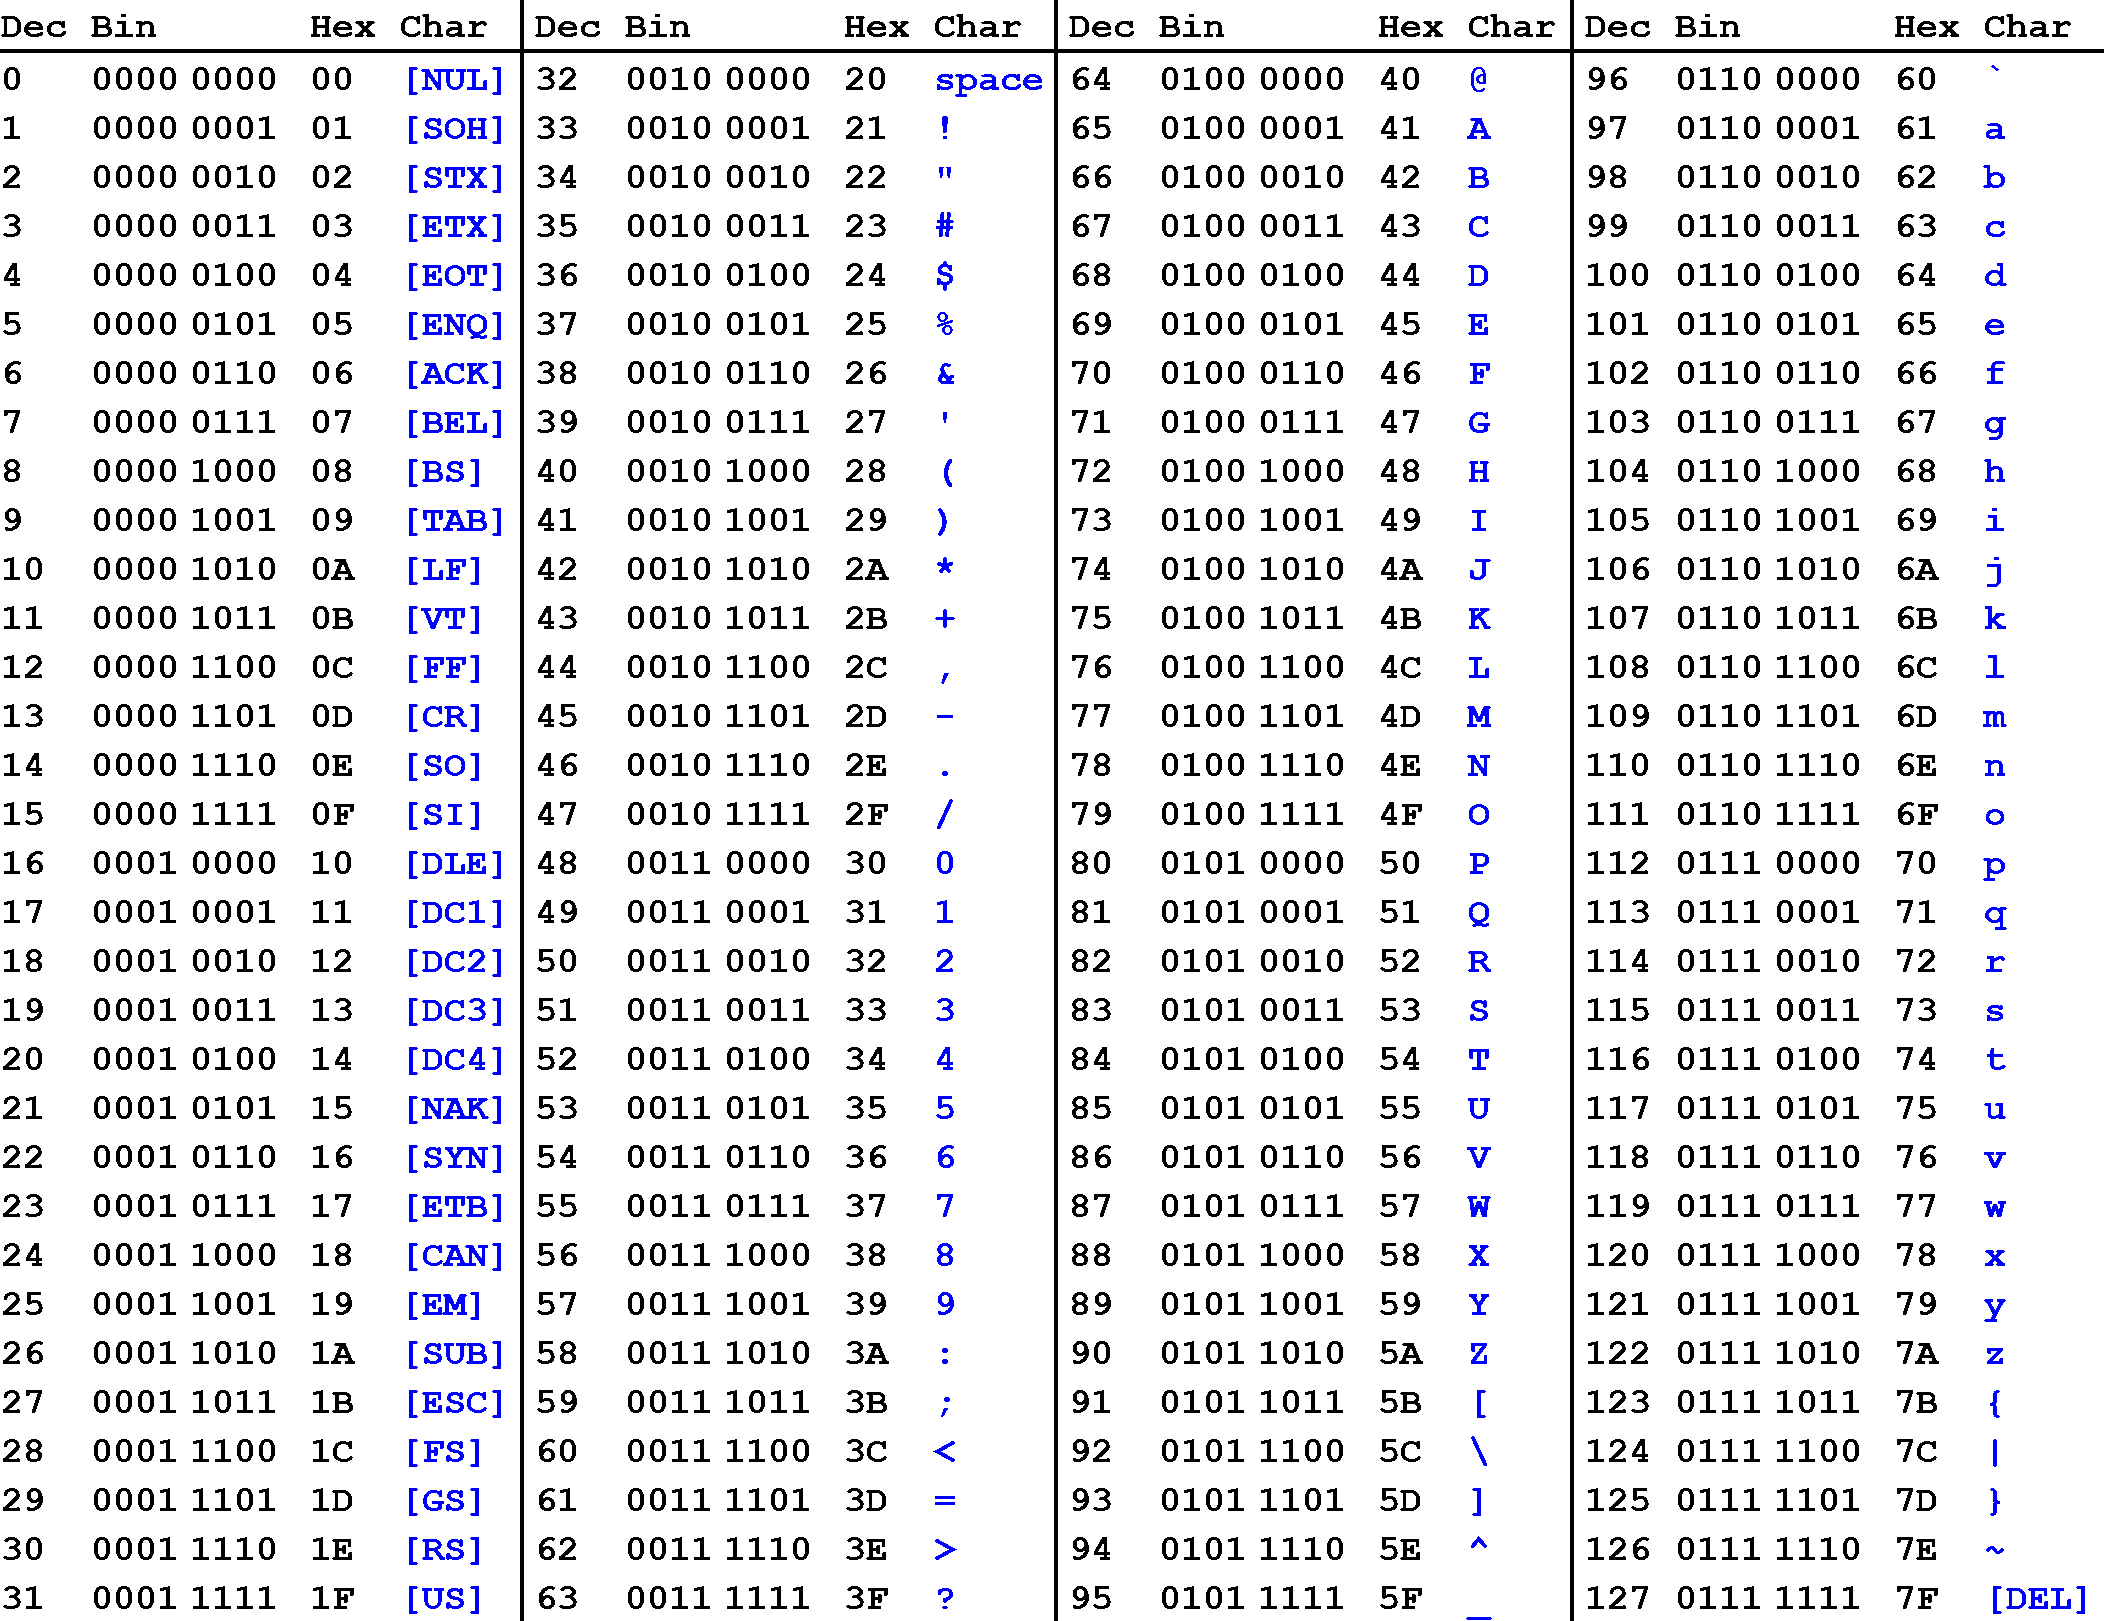
\includegraphics[width=425px]{ascii.png}\]

\end{document}